% arara: pdflatex: { action: nonstopmode }
% !arara: biber
% arara: pdflatex: { action: nonstopmode }
% arara: pdflatex: { action: nonstopmode }
% !arara: pdflatex: { action: nonstopmode }
% ----------------------------------------------------------------------------
% the XSIM package
% 
%   eXercise Sheets IMproved
% 
% ----------------------------------------------------------------------------
% Clemens Niederberger
% Web:    https://github.com/cgnieder/xsim
% E-Mail: contact@mychemistry.eu
% ----------------------------------------------------------------------------
% Copyright 2017 Clemens Niederberger
% 
% This work may be distributed and/or modified under the
% conditions of the LaTeX Project Public License, either version 1.3
% of this license or (at your option) any later version.
% The latest version of this license is in
%   http://www.latex-project.org/lppl.txt
% and version 1.3 or later is part of all distributions of LaTeX
% version 2005/12/01 or later.
% 
% This work has the LPPL maintenance status `maintained'.
% 
% The Current Maintainer of this work is Clemens Niederberger.
% ----------------------------------------------------------------------------
% If you have any ideas, questions, suggestions or bugs to report, please
% feel free to contact me.
% ----------------------------------------------------------------------------
\documentclass{xsim-manual}

\usepackage{filecontents}
\begin{filecontents*}{\jobname.bib}
@online{texsx:romannumeral,
  author = {Bruno Le Floch} ,
  title = {Cunning (La)TeX tricks} ,
  urldate = {2017-03-02} ,
  url = {http://tex.stackexchange.com/a/19769/}
}
@online{texsx:tagged/exsheets,
  title = {Questions tagged `exsheets'} ,
  author = {various} ,
  url = {http://tex.stackexchange.com/questions/tagged/exsheets} ,
  urldate = {2017-05-15}
}
\end{filecontents*}
\addbibresource{\jobname.bib}

\begin{document}

\section{Licence, Requirements and \textsc{readme}}
\license

\xsim\ loads the packages \pkg{expl3}~\cite{bnd:l3kernel},
\pkg{xparse}~\cite{bnd:l3packages}, \pkg{etoolbox}~\cite{pkg:etoolbox},
\pkg{array}~\cite{pkg:array} \pkg{booktabs}~\cite{pkg:booktabs} and
\pkg{translations}~\cite{pkg:translations}.  All of these packages are present
on a modern and up to date \TeX\ distribution such as \TeX~Live or MiK\TeX\ so
no further action should be needed.  When you are using \xsim\ you should be
using an up to date \TeX\ distribution, anyway.

\begin{bewareofthedog}
  Newer versions of \xsim\ may depend on newer versions of the support
  packages.  Remember: it is always dangerous to update single packages.
  Always update your \TeX\ distribution if you want an up to date version of a
  package.  Be careful: if you're in the middle of an important project it
  might be better to wait with the update until you've finished the project.
  Every update might be breaking some things.
\end{bewareofthedog}

\section{Motivation and Background}

It has been quite a while since I first published
\pkg{exsheets}~\cite{pkg:exsheets} in June 2012.  Since then it has gained a
user base and a little bit of popularity as the number of questions on tex.sx
shows (103~at the time of writing)~\cite{texsx:tagged/exsheets}.  User
questions, bug reports and feature requests improved it over the time.  It
still has a version number starting with a zero, though, which in my
versioning system means I still consider it experimental.

This is due to several facts.  It lacks a few features which I consider
essential for a full version~1.  For one thing it is not possible to have
several kinds of exercises numbered independently.  Using verbatim material
such as listings inside exercises and solutions is not possible and the
current workaround isn't that ideal either.  One request which dates back
quite a while now was to have different types of points to exercises\ldots

All of those aren't easy to add due to the way \pkg{exsheets} is implemented
right now. As a consequence I wanted to re-implement \pkg{exsheets} for a long
time.  This is what lead to \xsim.  Internally the package works completely
different.

\begin{bewareofthedog}
  \xsim\ will be the official successor of \pkg{exsheets} which is now
  considered obsolete but will stay alive and will still receive bugfix
  releases. However, new features will not be added to \pkg{exsheets} any
  more.
\end{bewareofthedog}

\section{How to Read the Manual}\label{sec:how-read-manual}

\subsection{Nomenclature}

Throughout this manual certain terms are used.  This section explains their
meaning in this manual.

\acuseall
\printacronyms[heading=none]

\subsection{Package Options}\label{sec:package-options}
\xsim\ has these package options:
\begin{options}
  \opt{verbose}
    Writes extensive information about what \xsim\ is doing into the log
    file.
  \opt{final}
    If used the exercise and solution environments will not rewrite the
    environment body files.
  \opt{clear-aux}
    If used every time the  total number of exercise changes \xsim\ will write
    \emph{less} information to the auxfile on the next run and only if the
    number of exercises stays stable between compilations the needed
    information will be written to the auxfile. \emph{This needs more
      compilations until everything stabilizes but should reduce the
      probability of possibly faulty exercises after changes to the document.}
    The \option{final} option automatically disables this option.  See also
    sections~\vref{sec:how-exerc-envir} and~\vref{sec:resolve-getting}.
\end{options}

Those options are used the usual way as package option
\begin{sourcecode}
  \usepackage[verbose]{xsim}
\end{sourcecode}
or as global option
\begin{sourcecode}
  \documentclass[verbose]{article}
\end{sourcecode}
or via the setup command:
\begin{commands}
  \command{xsimsetup}[\marg{options}]
    Set up \xsim's package options and all other options described at
    other places in the manual.
\end{commands}

\subsection{Setting Options}
Apart from the package options already described in
section~\vref{sec:package-options} \xsim\ has further options. Those can be
\enquote{toplevel} options or options belonging to a module.
\begin{options}
  \keyval*{toplevel}{value}
    A toplevel option.
  \keyval*{sublevel}{value}\Module*{module}
    A sublevel option belonging to the module \module*{module}
\end{options}
Both kinds of options are set with \cs{xsimsetup}:
\begin{sourcecode}
  \xsimsetup{
    toplevel = {value} ,
    module/sublevel = {value}
  }
\end{sourcecode}

\subsection{Command descriptions}

Some commands do have a \expandablesymbol\ symbol printed next to their
names.  This indicates that the command is expandable, \ie, it is usable in an
\cs*{edef} or \cs*{write} context and will expand according to its
description.  All other commands are engine protected, \ie, in the sense of
\eTeX's \cs*{protected}.

Some command name descriptions end with \code{\TF}.
\begin{commands}
  \command*{SomeCommand\TF}[\meta{arguments}\marg{true}\marg{false}]
    A command with maybe some arguments and ending with the two arguments
    \meta{true} and \meta{false}.
\end{commands}
This means two things: the command is a conditional which tests something and
depending on the outcome of the test leaves either the \meta{true} argument
(\code{T}) or the \meta{false} argument (\code{F}) in the input stream.  It
also means two additional commands exist:
\begin{commands}
  \command*{SomeCommandT}[\meta{arguments}\marg{true}]
    The same as \cs*{SomeCommandTF} but only with the \meta{true} argument and
    no \meta{false} argument.
  \command*{SomeCommandF}[\meta{arguments}\marg{false}]
    The same as \cs*{SomeCommandTF} but only with the \meta{false} argument and
    no \meta{true} argument.
\end{commands}


\section{Exercises and Solutions}

The two predefined environments for exercises and solutions are the following
ones:
\begin{environments}
  \environment{exercise}[\oarg{\acsp*{prop}}]
    Input and typeset an exercise.  See section~\vref{sec:exercise-properties}
    for details on exercise \acsp*{prop}.
  \environment{solution}[\oarg{options}]
    Input and typeset the solution to the exercise of the previous
    \env{exercise} environment.  See section~\vref{sec:printing-solutions} for
    details on options of solutions.
\end{environments}

\begin{example}
  \begin{exercise}
    A first example for an exercise.
  \end{exercise}
  \begin{solution}
    A first example for a solution.
  \end{solution}
\end{example}

As can be seen in the example a solution is not printed with the default
setup.  This can be changed using the following option.
\begin{options}
  \keybool{print}\Module{solution}\Default{false}
    Set if solutions are printed or or not.
\end{options}

The option (belonging to the module \module*{solution}) can either be set
locally as option to the \env{solution} environment
\begin{sourcecode}
  \begin{solution}[print=true]
    A first example for a solution.
  \end{solution}
\end{sourcecode}
or with the setup command for all following solutions:
\begin{sourcecode}
  \xsimsetup{
    solution/print = true
  }
\end{sourcecode}

There is an completely analoguous option for the \env{exercise} environment:
\begin{options}
  \keybool{print}\Module{exercise}\Default{true}
    Set if exercises are printed or or not.
\end{options}
More details on those two environments can be found in
section~\vref{sec:using-printing}.

\section{How the Exercise Environments Work}\label{sec:how-exerc-envir}
Both enviroments write the contents of their bodies verbatim to external files
following a certain naming structure:
\begin{itemize}
  \item
  \code{\meta{jobname}-\meta{type}-\meta{id}-exercise|solution-body.tex} 
\end{itemize}
The name starts with the name of the job (which is the name of the document
itself) followed by type and id of the corresponding exercise and then
followed by the environment type.  For example both enviroments from the first
example have been written to files named
\begin{itemize}
  \item \verbcode+xsim_manual-exercise-1-exercise-body.tex+ and
  \item \verbcode+xsim_manual-exercise-1-solution-body.tex+, respectively.
\end{itemize}
Details on the \meta{type} of an exercise will be given in
section~\vref{sec:new-exercise-types}.  \emph{The \meta{id} of an exercise is
  a positive integer unique to each exercise environment regardless if the
  exercise is being printed or used at all.}

These external files are input when the respective exercise or solution is
printed.  An advantage of using external files is that \emph{verbatim material
  is allowed} inside the environments.  Each of those files contains some
information about itself and where and why it was generated\footnote{In this
  example the sourcecode line number is misleading as the example where the
  file was generated itself was an external file where the \env{exercise}
  environment indeed \emph{was} on line~1.}:

\inputsourcecode{exercises/xsim_manual-exercise-1-exercise-body.tex}

Arguably one downside of the approach using external files for each exercise
and its solution is that your project folder will be cluttered with files.  In
order to deal with this somehow \xsim\ offers the following option:
\begin{options}
  \keyval{path}{path name}\Default
    With this option a subfolder or path within the main project folder can be
    given.  Exercises will be written to and included from this path.
    \emph{The path must exist on your system before you can use it!} This
    document uses \keyis{path}{exercises}.
  \keyval{file-extension}{string}\Default{\code{tex}}
    \sinceversion{0.10}This option let's you choose the extension of the
    auxiliary files.
\end{options}

Another thing to keep in mind: the environment in many ways works the same way
as the \env{filecontents}. \emph{This also means that you \emph{cannot} have
  comments on the first line of the environments:}
\begin{sourcecode}
  \begin{exercise}[points=2] % this will cause trouble
    Lorem ipsum
  \end{exercise}
\end{sourcecode}

\begin{bewareofthedog}
  \xsim\ writes a lot of stuff to the auxfile for re-using information on
  subsequent compilations.  If you add exercises, change properties \etc\ it
  might happen that wrong information is staying in the auxfile and is wrongly
  used by \xsim.  In such cases deleting the auxfile and doing a few fresh
  compilations may resolve your problems.

  Sometimes the \emph{existence of exercise or solution files from earlier
    compilations} may lead to wrong lists of exercises or solutions.  In such
  cases it can be useful to delete all those files and doing a fresh
  compilation.  It may be helpful to use a subfolder for those exernal files
  which will make deleting them a little bit easier. (Don't forget to both
  create the subfolder and set \option{path} accordingly then.)

  Using the \option{clear-aux} option might help to reduce erroneous exercises.
\end{bewareofthedog}

\section{New Exercise Types}\label{sec:new-exercise-types}

It is easy to define new exercise environments together with a corresponding
solution environment using the following command:
\begin{commands}
  \command{DeclareExerciseType}[\marg{type}\marg{parameters}]
    Declare a new exercise type analoguous to the \env{exercise} and
    \env{solution} environments.
\end{commands}
Declaring a new exercise type will also define a new command:
\begin{commands}
  \command{numberof\meta{exercise-env}s}
    These commands hold the absolut number of used exercises of type
    \meta{type}.  The meaning of \meta{exercise-env} will become clear below
    when the exercise parameters are explained.  It is always the same as the
    exercise environment name.
\end{commands}
\begin{example}
  There are \numberofexercises~exercises and \numberofproblems~problem in this
  manual.
\end{example}
\xsim's pre-defined environment pair has been defined as follows:
\begin{sourcecode}
  \DeclareExerciseType{exercise}{
    exercise-env      = exercise ,
    solution-env      = solution ,
    exercise-name     = \XSIMtranslate{exercise} ,
    solution-name     = \XSIMtranslate{solution} ,
    exercise-template = default ,
    solution-template = default
  }
\end{sourcecode}

The above already is an example for almost all parameters that can (and often
must) be set.  Here is the complete list:
\begin{parameters}
  \paraval{exercise-env}{exercise environment name}
    The name for the environment used for the exercises of type \meta{type}.
    \emph{This parameter is mandatory.} It can't be changed afterwards.
  \paraval{solution-env}{solution environment name}
    The name for the environment used for the solutions of type \meta{type}.
    \emph{This parameter is mandatory.} It can't be changed afterwards.
  \paraval{exercise-name}{exercise name}
    The name of the exercises of type \meta{type} -- used for typesetting.
    \emph{This parameter is mandatory.}
  \paraval{solution-name}{solution name}
    The name of the solutions of type \meta{type} -- used for typesetting.
    \emph{This parameter is mandatory.}
  \paraval{exercise-template}{exercise template}
    The template used for typesetting the exercises of type \meta{type}.
    \emph{This parameter is mandatory.} See
    section~\vref{sec:styl-exerc-templ} for details on templates.
  \paraval{solution-template}{solution template}
    The template used for typesetting the exercises of type \meta{type}.
    \emph{This parameter is mandatory.} See
    section~\vref{sec:styl-exerc-templ} for details on templates.
  \paraval{counter}{counter name}
    The counter used for the exercises of type \meta{type}.  If not explicitly
    set the counter with the same name as \parameter{exercise-env} is used.
    Otherwise the specified counter is used.  This enables to have different
    types of exercises sharing a common counter.  \emph{This parameter can't
      be changed afterwards.}  If the explicit or implicit counter does not
    exist, yet, it will be defined.
  \paraval{solution-counter}{counter name}
    The counter used for the solutions of type \meta{type}.  If not explicitly
    set the counter with the same name as \parameter{solution-env} is used.
    Otherwise the specified counter is used.  This enables to have different
    types of solutions sharing a common counter although this doesn't actually
    make much sense.  But it can be useful to avoid using an already existing
    counter. \emph{This parameter can't be changed afterwards.}  If the
    explicit or implicit counter does not exist, yet, it will be defined.  The
    sole purpose of this counter is to be able to label solutions so they can
    be \cs*{pageref}ed.
  \paraval{number}{integer}
    An internal parameter that is used to keep track of the number of
    exercises of a type.  This parameter cannot be set or changed by the
    user.
\end{parameters}

It is possible to change some of the parameters after an exercise type has
been defined.  Those include \parameter{exercise-name},
\parameter{solution-name}, \parameter{exercise-template}, and
\parameter{solution-template}:
\begin{commands}
  \command{SetExerciseParameter}[\marg{type}\marg{parameter}\marg{value}]
    Usable to set a single parameter to a new value.
  \command{SetExerciseParameters}[\marg{type}\marg{parameters}]
    Set several parameters at once. \meta{parameters} is a csv list of
    key/value pairs.
\end{commands}
If you try to set an already set but fixed parameter like
\parameter{exercise-env} a warning will be written to the log file.  For all
parameters that can be changed also options exist wich can be set via
\cs{xsimsetup}.  They are explained in
section~\vref{sec:environment-options-hooks}.

\begin{bewareofthedog}
  All exercises of a type use the parameters
  (\eg, \parameter{exercise-template}) that are \emph{currently active}.  If
  you want exercises with a different look or different names in the same
  document you should use different exercises types.
\end{bewareofthedog}

\section{Exercise Properties}\label{sec:exercise-properties}

\subsection{Predefined Properties}

Exercise like the \env{exercise} environment and possibly others defined with
\cs{DeclareExerciseType} have a number of predefined \acsp*{prop}:
\begin{properties}
  \propval{id}{integer}
    Holds the internal id of an exercise.  \emph{Cannot be set by the user}.
  \propval{ID}{text}
    Holds the user id of an exercise if defined.  Otherwise it is equal to
    \property{id}.
  \propval{counter}{text}
    Holds the counter value represenation of an exercise (\ie, what you
    usually know as \cs*{the\meta{counter}}).  \emph{Cannot be set by the
      user}.
  \propval{counter-value}{integer}
    Holds the counter value of an exercise (\ie, what you usually know as
    \cs*{arabic}\marg{counter}).  \emph{Cannot be set by the user}.
  \propval{subtitle}{text}
    Holds the subtitle of an exercise.
  \propval{points}{number}
    Holds the reachable points of an exercise.
  \propval{bonus-points}{number}
    Holds the reachable bonus-points of an exercise.
  \propbool{print}
    Holds the print boolean of an exercise.
  \propbool{print\bang}
    Holds a special print boolean of an exercise, see
    page~\pageref{property:print!}.
  \propbool{use}
    Holds the usage boolean of an exercise.
  \propbool{use\bang}
    Holds a special usage boolean of an exercise, see
    page~\pageref{property:print!}.
  \propbool{used}
    True if an exercise has been used at least once.  For an existing exercise
    this is only false for exercises that have been collected
    (\cf~section~\vref{sec:collecting-exercises}).
  \propval{tags}{csv list of tags}
    Holds the list of tags the exercise should be associated with.
  \propval{topics}{csv list of topics}
    Holds the list of topics the exercise should be associated with.
  \propval{page}{text}
    Holds the page counter value represenation of an exercise (\ie, what you
    usually know as \cs*{thepage}).
  \propval{page-value}{integer}
    Holds the page counter value of an exercise (\ie, what you usually know as
    \cs*{arabic}\Marg{page}).
  \propval{section}{text}
    Holds the section counter value represenation of an exercise (\ie, what
    you usually know as \cs*{thesection}).
  \propval{section-value}{integer}
    Holds the section counter value of an exercise (\ie, what you usually know
    as \cs*{arabic}\Marg{section}).
  \propval{chapter}{text}
    Holds the chapter counter value represenation of an exercise (\ie, what
    you usually know as \cs*{thechapter}).  \emph{Only if a command
      \cs*{chapter} \emph{and} a counter \code{chapter} exist.}
  \propval{chapter-value}{integer}
    Holds the chapter counter value of an exercise (\ie, what you usually know
    as \cs*{arabic}\Marg{chapter}).  \emph{Only if a command \cs*{chapter}
      \emph{and} a counter \code{chapter} exist.}
  \propval{sectioning}{section numbers}
    Holds five brace groups which in turn hold the section numbers (integers)
    of the exercise in the order
    \marg{chapter}\marg{section}\marg{subsection}\marg{subsubsection}\marg{paragraph}.
\end{properties}

Some of these \acsp*{prop} are fixed and cannot be set by the user.  Those
include \property{id}, \property{counter}, and \property{counter-value}.  The
others can be set using the optional argument of the exercise environment.

\begin{example}
  \begin{exercise}[subtitle={This is a subtitle},points=4,bonus-points=1]
    An exercise where some properties have been set.
  \end{exercise}
\end{example}

\subsection{Declaring Own Properties}

\xsim\ offers the possibility to declare additional exercise properties:
\begin{commands}
  \command{DeclareExerciseProperty}[\barg\sarg\narg\marg{property}]
    Declares the property \meta{property}.
    
    If used with the optional \barg\ a \textbf{unique property} is defined
    which means that each exercise must have a property value distinct from
    all other exercises (all means all -- \emph{independent from the exercise
      type}).

    If used with the optional \sarg\ a \textbf{boolean property} is defined
    which means that it only should get the values \code{true} or \code{false}
    and if used without value it gets the value \code{true} instead of an
    empty value.  If any other value is used the property is set to
    \code{false}.  A boolean property obviously cannot be unique.  The
    optional \sarg\ takes precedence over the optional \barg, \ie, if both are
    present the property is boolean \emph{but not} unique.

    If used with the optional \narg\ a property is defined which won't get
    updated through subsequent compilation runs but is only set when the
    exercise is used.
  \command{DeclareExercisePropertyAlias}[\marg{property 1}\marg{property 2}]
    Declares \meta{property 1} to be an alias of \meta{property 2}.  This
    means that each time \meta{property 2} is set \meta{property 1} will be
    set to the same value \emph{unless} it has been set already.  As an
    example: property \property{ID} is an alias of property \property{id}.
\end{commands}

This is better demonstrated with an example:
\begin{example}
  \begin{exercise}
    \lipsum[4] % from package `lipsum'
    \verb+\GetExerciseProperty{id}+: \GetExerciseProperty{id} \par
    \verb+\GetExerciseAliasProperty{ID}+: \GetExerciseAliasProperty{ID} \par
    \verb+\GetExerciseProperty{ID}+: \GetExerciseProperty{ID}
  \end{exercise}
  \begin{exercise}[ID=foo-bar]
    \lipsum[4]
    \verb+\GetExerciseProperty{id}+: \GetExerciseProperty{id} \par
    \verb+\GetExerciseAliasProperty{ID}+: \GetExerciseAliasProperty{ID} \par
    \verb+\GetExerciseProperty{ID}+: \GetExerciseProperty{ID}
  \end{exercise}
\end{example}

The power of properties will get more clear when reading
section~\vref{sec:styl-exerc-templ} about templates.

\subsection[Exercise Goals]{A Special Kind of Property: Exercise Goals}\label{sec:goals}

Exercise goals are a generic concept in \xsim\ for exercise properties like
\property{points} or \property{bonus-points}.  Those are properties which can
(only) get a decimal number as value the sum of which is calculated and
available (after a compilation) throughout the document.
\begin{commands}
  \command{DeclareExerciseGoal}[\marg{goal}]
    Declare a new exercise goal named \meta{goal} and also a property called
    \meta{goal}.
  \command{TotalExerciseTypeGoal}[\marg{type}\marg{goal}\marg{singular}\marg{plural}]
    Get the sum of goal \meta{goal} for all exercises of type \meta{type}.
    \meta{singular} and \meta{plural} are placed after the sum in the input
    stream depending on whether the sum equals~$1$ or not.
    \command{TotalExerciseTypeGoals}[\marg{type}\marg{list of
      goals}\marg{singular}\marg{plural}]
    Get the sum of goal all goals in \meta{list of goals} for all exercises of
    type \meta{type}.  The goal names in \meta{list of goals} must be
    separated with \code{+}. \meta{singular} and \meta{plural} are placed
    after the sum in the input stream depending on whether the sum equals~$1$
    or not.
  \command{TotalExerciseGoal}[\marg{goal}\marg{singular}\marg{plural}]
    Get the sum of goal \meta{goal} for all exercises. \meta{singular} and
    \meta{plural} are placed after the sum in the input stream depending on
    whether the sum equals~$1$ or not.
  \command{TotalExerciseGoals}[\marg{list of
    goals}\marg{singular}\marg{plural}]
    Get the sum of goal all goals in \meta{list of goals} for all exercises.
    The goal names in \meta{list of goals} must be separated with
    \code{+}. \meta{singular} and \meta{plural} are placed after the sum in
    the input stream depending on whether the sum equals~$1$ or not.
  \command{AddtoExerciseTypeGoal}[\marg{type}\marg{goal}\marg{value}]
    Adds \meta{value} to the goal \meta{goal} of exercise type \meta{type}.
  \command{AddtoExerciseTypeGoalPrint}[\marg{type}\marg{goal}\marg{value}%
    \marg{singular}\marg{plural}]
    Adds \meta{value} to the goal \meta{goal} of exercise type \meta{type}.
    The value and -- depending on wether the value equals $1$ or not --
    \meta{singular} or \meta{plural} are left in the input stream.
  \command{AddtoExerciseGoal}[\marg{goal}\marg{value}]
    Adds \meta{value} to the goal \meta{goal} of the current exercise
    type. (To be used within exercises.)
  \command{AddtoExerciseTypeGoalPrint}[\marg{goal}\marg{value}%
    \marg{singular}\marg{plural}]
    Adds \meta{value} to the goal \meta{goal} of the current exercise type.
    The value and -- depending on wether the value equals $1$ or not --
    \meta{singular} or \meta{plural} are left in the input stream. (To be used
    within exercises.)
  \command{ExerciseGoalValuePrint}[\marg{value}\marg{singular}\marg{plural}]
    Print \meta{value} and -- depending on wether the value equals $1$ or not --
    \meta{singular} or \meta{plural}.
  \command{printgoal}[\marg{value}]
    Print \meta{value} according to option \option{goal-print}.  Defined in
    terms of \cs{ExerciseGoalValuePrint}.
  \command{printpoints}[\marg{type}]
    Print the sum of points for all exercises of type \meta{type} followed by
    an appropriate translation of the words \enquote{point} or
    \enquote{points}, respectively\footnote{See section~\vref{sec:exerc-transl}
      for details on the definition and usage of language dependent words.}.
    Defined in terms of \cs{TotalExerciseTypeGoal}.
  \command{printtotalpoints}
    Print the sum of points for all exercises followed by an appropriate
    translation of the words \enquote{point} or \enquote{points},
    respectively.  Defined in terms of \cs{TotalExerciseGoal}.
  \command{addpoints}[\sarg\marg{value}]
    Adds \meta{value} to the points of the current exercise type. (To be used
    within exercises.)  Prints the value followed by an appropriate
    translation of the words \enquote{point} or \enquote{points},
    respectively.  The starred version prints nothing.  Defined in terms of
    \cs{AddtoExerciseGoal} and \cs{AddtoExerciseGoalPrint}.
  \command{points}[\marg{value}]
    Print \meta{value}followed by an appropriate translation of the words
    \enquote{point} or \enquote{points}, respectively.  Defined in terms of
    \cs{ExerciseGoalValuePrint}.
  \command{printbonus}[\marg{type}]
    Print the sum of bonus points for all exercises of type \meta{type}
    followed by an appropriate translation of the words \enquote{point} or
    \enquote{points}, respectively.  Defined in terms of
    \cs{TotalExerciseTypeGoal}.
  \command{printtotalbonus}
    Print the sum of bonus points for all exercises followed by an appropriate
    translation of the words \enquote{point} or \enquote{points},
    respectively.  Defined in terms of \cs{TotalExerciseGoal}.
  \command{addbonus}[\sarg\marg{value}]
    Adds \meta{value} to the bonus points of the current exercise type. (To be
    used within exercises.)  Prints the value followed by an appropriate
    translation of the words \enquote{point} or \enquote{points},
    respectively.  The starred version prints nothing.  Defined in terms of
    \cs{AddtoExerciseGoal} and \cs{AddtoExerciseGoalPrint}.
\end{commands}

The two existing goals are defined with
\begin{sourcecode}
  \DeclareExerciseGoal{points}
  \DeclareExerciseGoal{bonus-points}
\end{sourcecode}

When goal values are printed the decimal number is fed to a function which can
be changed using the following option:
\begin{options}
  \keyval{goal-print}{code}\Default{\#1}
    How to format goal values.  Use \code{\#1} to refer to the actual number.
\end{options}

At last some examples for a custom command: let's say you want a command which
prints the complete sum for all exercises of all exercise types of both
\property{points} \emph{and} \property{bonus-points} added up:
\begin{sourcecode}
  \NewDocumentCommand\printsumofpointsandbonus{}{%
    \TotalExerciseGoals{points+bonus-points}
      {\,\XSIMtranslate{point}}
      {\,\XSIMtranslate{points}}%
  }
\end{sourcecode}
Here is how you could mimick the command \cs*{totalpoints} from
\pkg{exsheets}:
\begin{sourcecode}
  \NewDocumentCommand\pointsandbonus{}{%
    \TotalExerciseGoal{points}{}{}%
    \IfExerciseGoalsSumF{bonus-points}{=0}
      {\,(+\,\TotalExerciseGoal{bonus-points}{}{})}%
    \,\XSIMtranslate{points}%
  }
\end{sourcecode}


\subsection[Exercise Tags]{A Special Kind of Property: Exercise Tags}\label{sec:tags}

Exercise tags are a generic concept in \xsim\ for exercise properties like
\property{tags} or \property{topics}.  Those are properties which can (only)
get a csv list of strings as value.  Those strings can be used to selectively
use exercises.  See section~\vref{sec:using-printing} for details on
\emph{usage} of exercises and the difference to \emph{printing} an exercise
and how to use exercise tags for selection.
\begin{commands}
  \command{DeclareExerciseTagging}[\marg{tag}]
    This defines an exercise tagging group named \meta{tag}.  It also defines a
    property named \meta{tag}.  In addition two options are defined: an option
    named \code{\meta{tag}} which can be used for selection and an boolean
    option \code{\meta{tag}/ignore-untagged}.
\end{commands}
The two existing tagging groups have been defined and preset with the
following code:
\begin{sourcecode}
  \DeclareExerciseTagging{tags}
  \DeclareExerciseTagging{topics}
  \xsimsetup{tags/ingore-untagged=false}
\end{sourcecode}
This means that these options are available:
\begin{options}
  \keyval{tags}{csv list of tags}
    Choose the set of tags whose associated exercises should be printed.
  \keyval{topics}{csv list of topics}
    Choose the set of topics whose associated exercises should be printed.
  \keybool{ignore-untagged}\Module{tags}\Default{false}
    If set to true exercises with no tags will be printed even if tags have
    been chosen with the option \option{tags}.
  \keybool{ignore-untagged}\Module{topics}\Default{true}
    If set to true exercises with no topics will be printed even if topics
    have been chosen with the option \option{topics}.
\end{options}

It may happen that you choose certain tags for printing and want one or two
exercises to be printed or used even if they don't match the tagging
criteria.  For this reason two additional properties exist which can be set to
an exercise:\label{property:print!}
\begin{properties}
  \propbool{print\bang}
    If set to true the exercise will be printed (and thus used) regardless of
    other conditions.
  \propbool{use\bang}
    If set to true the exercise will be used regardless of other conditions.
\end{properties}

\section{Using and Printing an Exercise}\label{sec:using-printing}
\subsection{What the Environments do}

When an exercise is started with \environ{exercise} (or other environments
defined through \cs{DeclareExerciseType}) then different things happen
depending on different settings:
\begin{itemize}
  \item If the \emph{insert mode} is active nothing happens, see
    section~\vref{sec:collecting-exercises} for details on this.
  \item Else the id integer is incremented.
  \item If the exercise is \emph{used} the corresponding counter is stepped
    and the exercise is added to the \enquote{use list}.  The properties
    \property{counter} and \property{use} are updated accordingly.
  \item If an exercise is \emph{printed} then it is also \emph{used}. An
    exercise that isn't used cannot be printed.  Being printed means two
    things: being added to the \enquote{print list} and being typeset at the
    position where the exercise is placed in the source file.  If an exercise
    is \emph{not printed but used} it means that the counter will be stepped.
    This can be useful for creating an exercise sheet only containing the
    solutions for some exercises.
  \item If an exercise is printed certain hooks and template code is inserted
    around the environment body.
\end{itemize}

\begin{example}
  \begin{exercise}[print=false]
    This exercise will not be printed but the exercise counter will be
    incremented nonetheless. Its solution will be printed in the list of
    solutions.
  \end{exercise}
  \begin{solution}
    The solution of the exercise that has not been printed.
  \end{solution}
\end{example}

The schematic structure of an exercise is shown in
figure~\vref{fig:schematic-structure}.

\begin{figure}
  \centering
  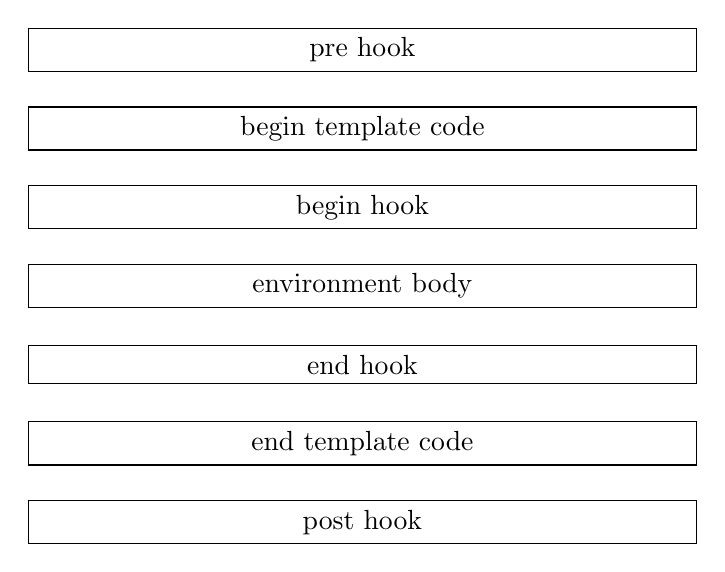
\begin{tikzpicture}
    \node[draw,minimum width=.7\linewidth] at (0,0)  {pre hook};
    \node[draw,minimum width=.7\linewidth] at (0,-1) {begin template code};
    \node[draw,minimum width=.7\linewidth] at (0,-2) {begin hook};
    \node[draw,minimum width=.7\linewidth] at (0,-3) {environment body};
    \node[draw,minimum width=.7\linewidth] at (0,-4) {end hook};
    \node[draw,minimum width=.7\linewidth] at (0,-5) {end template code};
    \node[draw,minimum width=.7\linewidth] at (0,-6) {post hook};
  \end{tikzpicture}
  \caption{Schematic structure of an exercise or solution.}\label{fig:schematic-structure} 
\end{figure}

\subsection{Environment Options \& Hooks}\label{sec:environment-options-hooks}

For each exercise type there are the following options for both environments,
the environments' names are the module names for the options (here using the
\enquote{exercise} type):
\begin{options}
  \keybool{print}\Module{exercise}\Default{true}
    Determines if exercises of type \enquote{exercise} are printed.
  \keybool{use}\Module{exercise}\Default{true}
    Determines if exercises of type \enquote{exercise} are used.
  \keyval{within}{counter}\Module{exercise}\Default
    Adds the exercise counter to the reset list of the counter
    \meta{counter}.  \emph{Beware that if the counter is a shared counter
      this will affect \emph{all objects} using this counter!}
  \keyval{the-counter}{code}\Module{exercise}
    An interface for redefining the counter representation command
    \cs*{the\meta{counter}}.
  \keyval{template}{template}\Module{exercise}
    An interface for \cs{SetExerciseParameter}\Marg{exercise}%
    \Marg{exercise-template}\marg{template}.
  \keyval{template}{template}\Module{solution}
    An interface for \cs{SetExerciseParameter}\Marg{exercise}%
    \Marg{solution-template}\marg{template}.
  \keyval{name}{name}\Module{exercise}
    An interface for \cs{SetExerciseParameter}\Marg{exercise}%
    \Marg{exercise-name}\marg{name}.
  \keyval{name}{name}\Module{solution}
    An interface for \cs{SetExerciseParameter}\Marg{exercise}%
    \Marg{solution-name}\marg{name}.
  \keyval{pre-hook}{code}\Module{exercise}\Default
    The code for the \emph{pre exercise hook} for exercises of the type
    \enquote{exercise}.
  \keyval{begin-hook}{code}\Module{exercise}\Default
    The code for the \emph{begin exercise hook} for exercises of the type
    \enquote{exercise}.
  \keyval{end-hook}{code}\Module{exercise}\Default
    The code for the \emph{end exercise hook} for exercises of the type
    \enquote{exercise}.
  \keyval{post-hook}{code}\Module{exercise}\Default
    The code for the \emph{post exercise hook} for exercises of the type
    \enquote{exercise}.
  \keybool{print}\Module{solution}\Default{false}
    Determines if solutions of type \enquote{exercise} are printed.
  \keyval{pre-hook}{code}\Module{solution}\Default
    The code for the \emph{pre solution hook} for solutions of the type
    \enquote{exercise}.
  \keyval{begin-hook}{code}\Module{solution}\Default
    The code for the \emph{begin solution hook} for solutions of the type
    \enquote{exercise}.
  \keyval{end-hook}{code}\Module{solution}\Default
    The code for the \emph{end solution hook} for solutions of the type
    \enquote{exercise}.
  \keyval{post-hook}{code}\Module{solution}\Default
    The code for the \emph{post solution hook} for solutions of the type
    \enquote{exercise}.
  % TODO
\end{options}

\subsection{(Re-) Inserting a Certain Exercise}
If you know type and \property{id} of an exercise you can (re-)insert every
existing exercise, \ie, every exercise whose external file exists.
\begin{commands}
  \command{printexercise}[\marg{type}\marg{id}]
    Inserts the exercise of type \meta{type} with the \property{id}
    \meta{id}.
\end{commands}
\begin{example}
  \printexercise{exercise}{5}
\end{example}

\section{Collecting Exercises}\label{sec:collecting-exercises}

\subsection{Background}
\xsim\ knows the concept of \enquote{exercise collections}.  A collection of
exercises can be useful when you want to print a certain group of exercises
several times.  Each collection must have a unique name with which you can
refer to the corresponding collection.  A collection is realized by declaring
the collection and by surrounding the exercises belonging to the collection
with a certain pair of commands (this is explained in the next section).

Let's say you have several files of math exercises where one only contains
geometry exercises and another only calculus exercises and so on.  Surrounding
the \cs*{input} of each file with said pair of commands for a certain
collection all exercises of the corresponding file now are a collection which
then can be printed at once whereever you want the collection of exercises to
be printed.  By choosing certain tags (see section~\vref{sec:tags}) inside
each collection you could even cherry-pick exercises from the external file.

\subsection{Usage}
\emph{A collection must be declared in the preamble.}  Using a pair of
commands explained below exercises between those commands are added to the
corresponding collection but not printed.  After a collection is completed the
collection can be printed as often as needed.
\begin{commands}
  \command{DeclareExerciseCollection}[\marg{collection name}]
    Define a new collection \meta{collection name} in the document preamble.
  \command{collectexercisestype}[\marg{collection name}\marg{exercise type}]
    Opens the collection \meta{collection name} which now collects all
    exercises of type \meta{exercise type} until the collection is closed with
    \cs{collectexercisesstop}.  Collections of other types are not
    collected\footnote{This command starts a group with
      \cs*{begingroup}!}.
  \command{collectexercises}[\marg{collection name}]
    Opens the collection \meta{collection name} which now collects all
    exercises until the collection is closed with
    \cs{collectexercisesstop}\footnote{This command starts a group with
      \cs*{begingroup}!}.
  \command{collectexercisesstop}[\marg{collection name}]
    Closes the collection \meta{collection name}\footnote{This command ends
      a group with \cs*{endgroup}!}.
  \command{printcollection}[\oarg{options}\marg{collection name}]
    Prints the collection \meta{collection name}, \ie, all exercises collected
    earlier.  This command cannot be used before the corresponding collection
    has been closed correctly.
\end{commands}

Valid options are the following:
\begin{options}
  \keybool{headings}\Module{print-collection}\Default{false}
    If true a heading for each exercise type is inserted.
  \keyval{headings-template}{template}\Module{print-collection}\Default{collection}
    The heading template used when \keyis{headings}{true}.
  \keychoice{print}{exercises,solutions,both}\Module{print-collection}\Default{exercises}
    Determines wether \cs{printcollection} prints the exercises or the
    solutions of the collection.  When you choose \code{both} exercises and
    solutions are printed alternately.
\end{options}

Those options can also be set via \cs{xsimsetup} using the module
\module{print-collection}.

\begin{bewareofthedog}
  Please be aware that exercises are not used or printed while they are
  collected.  Nonetheless the property \property{use} is set to \code{true}
  (so that solutions can be printed even if the exercises are not) and the
  property \property{print} is set to \code{false}.  Also their counters are
  \emph{not stepped} during the process.  This only happens when they are
  printed the first time, \cf~the \property{used} property.  At that time
  also the properties \property{page}, \property{section} and
  \property{chapter} are set and the property \property{print} is set to
  \code{true}.
\end{bewareofthedog}

The usage should be clear:
\begin{example}
  \collectexercises{foo}
  \begin{exercise}
    This exercise is added to the collection `foo'.
  \end{exercise}
  \begin{exercise}
    This exercise is also added to the collection `foo'.
  \end{exercise}
  \begin{exercise}
    So is this.
  \end{exercise}
  \begin{exercise}
    As well as this one.
  \end{exercise}
  \collectexercisesstop{foo}
\end{example}
Once the collection is closed it can be printed:
\begin{example}
  \printcollection{foo}
\end{example}

You can open several collections at the same time:
\begin{sourcecode}
  \collectexercises{foo}
    ...
  \collectexercisestype{bar}{exercises}
    ...
  \collectexercisesstop{bar}
    ...
  \collectexercisesstop{foo}
\end{sourcecode}
Exercises will be added to each open collection.

There is one generic collection called \enquote{\code{all exercises}}.  As the
name already suggests it will hold all exercises.  So if you say
\begin{sourcecode}
  \printcollection{all exercises}
\end{sourcecode}
all exercises will be printed.

\begin{bewareofthedog}
  If you use \cs*{label}s inside of exercises and you print exercises more
  than once in your document (by reusing a collection for example) you will
  get
\begin{sourcecode}
  LaTeX Warning: There were multiply-defined labels.
\end{sourcecode}
  Equally if you have environments like \environ{equation} which step a
  counter inside an exercise or solution the counter will be stepped each time
  the exercise is used.
\end{bewareofthedog}

At last now an example using external files, collections and tags:
\begin{sourcecode}
  % preamble:
  % \DeclareExerciseCollection{foo-easy}
  % \DeclareExerciseCollection{foo-medium}
  % \DeclareExerciseTagging{difficulty}

  % document:
  \collectexercises{foo-easy}
  \xsimsetup{difficulty=easy}
  \input{foo.tex}
  \collectexercisesstop{foo-easy}
  % collection `foo-easy' now contains all exercises of file `foo.tex' tagged
  % with `difficulty=easy'

  \collectexercises{foo-medium}
  \xsimsetup{difficulty=medium}
  \input{foo.tex}
  \collectexercisesstop{foo-medium}
  % collection `foo-medium' now contains all exercises of file `foo.tex'
  % tagged with `difficulty=medium'
\end{sourcecode}

\begin{bewareofthedog}
  The recommended usage is similar to the last example.  Actually a collection
  can be printed \emph{before} it is opened, too.  (This needs \emph{at least}
  two compilations, though.)  However, it is safer printing a collection only
  once and only \emph{after it has been collected}.  No guaranties are given
  that properties are set correctly if you use the collection before.  You
  usually also will make sure that the exercises in a collection are unique,
  \ie, that an exercise is not part of several collections -- at least not if
  both collections are printed in the same document.
\end{bewareofthedog}

\section{Printing Random Exercises From a Collection}
\xsim\ provides the possibility of selecting random exercises from a
collection (\cf~section~\vref{sec:collecting-exercises}).
\begin{commands}
  \command{printrandomexercises}[\oarg{options}\marg{number}]
    This command prints \meta{number} random exercises from the collection
    chosen with option \option{collection}, see below.  When this command is
    used it generates a random list of integers which is written to the
    \code{aux} file.  On the subsequent compilations the according exercises
    are printed.  \emph{If you want to regenerate the random list you have to
      delete the \code{aux} file before compiling.}
\end{commands}
Valid options for this command are:
\begin{options}
  \keybool{sort}\Module{random}\Default{true}
    Determines wether the random chosen exercises should be sorted according
    to their order of definition in the collection or not.
  \keyval{collection}{collection}\Module{random}\Default{all exercises}
    The collection from which the exercises are to be chosen from.
  \keyval{exclude}{csv list of ids}\Module{random}
    A list of \property{id}s or \property{ID}s of exercises \emph{not} to be
    chosen.
  \keychoice{print}{exercises,solutions,both}\Module{random}\Default{exercises}
    Determines wether \cs{printrandomexercises} prints the exercises or the
    solutions.  When you choose \code{both} exercises and solutions are
    printed alternately.
\end{options}

\begin{example}
  \printrandomexercises[collection=foo]{2}
\end{example}

The example above of course doesn't make much sense but if you have a
collection which collects exercises from an external file and the exercises
haven't been printed in the document before then you will get a list of
subsequently numbered exercises.

\section{Printing Solutions}\label{sec:printing-solutions}

There are different commands for printing the solutions to exercises:
\begin{commands}
  \command{printsolutionstype}[\sarg\oarg{options}\marg{exercise type}]
    Prints the solutions of all used exercises of type \meta{exercise type}.
    The starred version only prints the solutions of all printed exercises of
    type \meta{exercise type}.
  \command{printsolutions}[\sarg\oarg{options}]
    Prints the solutions of all used exercises of all types ordered by type.
    The starred version only prints the solutions of all printed exercises of
    all types.
  \command{printallsolutions}[\sarg\oarg{options}]
    Prints the solutions of all used exercises of all types ordered by
    appearance in the document.  The starred version only prints the solutions
    of all printed exercises of all types.
  \command{printsolution}[\oarg{options}\marg{type}\marg{id}]
    Prints the solution of the exercise of type \meta{type} with the
    \property{id} \meta{id}.
\end{commands}

\begin{example}
  \printsolutionstype{exercise}
\end{example}

The options can be divided into two groups.  The ones in the first group
modify the layout.
\begin{options}
  \keybool{headings}\Module{print-solutions}\Default{true}
    If true a heading for each exercise type is inserted.
  \keyval{headings-template}{template}\Module{print-solutions}\Default{default}
    The heading template used when \keyis{headings}{true}.
\end{options}

The ones in the second group set conditions selecting which solutions are
printed.  If you combine those conditions a solution is printed if it meets
either of the conditions.
\begin{options}
  \keychoice{section}{\default{true},false,\meta{integer}}\Module{print-solutions}%
    \Default{false}
    If you set \keyis{section}{true} only solutions of exercises of the
    current section are printed.  If you set \keyis{section}{4} only solutions
    of exercises in a section with number~$4$ are printed.
  \keychoice{chapter}{\default{true},false,\meta{integer}}\Module{print-solutions}%
    \Default{false}
    If you set \keyis{chapter}{true} only solutions of exercises of the
    current chapter are printed.  If you set \keyis{chapter}{4} only solutions
    of exercises in a chapter with number~$4$ are printed.
  \keychoice{collection}{false,\meta{collection name}}\Module{print-solutions}%
    \Default{false}
    If used only solutions of exercises belonging to collection
    \meta{collection name} are printed.
\end{options}

The conditions can be combined.  The following call will only print solutions
from exercises in section~3 of chapter~2:
\begin{sourcecode}
  \printsolutions[chapter=2,section=3]
\end{sourcecode}

\begin{bewareofthedog}
  The selection per section or per chapter relies on the \emph{counter
    numbers} of the sections or chapters, respectively.  This means if section
  numbers are reset (\eg\ by \cs*{chapter} or \cs*{appendix}) and you have
  exercises from \emph{different} sections with \emph{the same section number}
  the solutions of \emph{all those exercises} will be printed.  This means you
  only should use the \option{section} selection when section are the top
  document level headings (apart from parts) and you have no exercises in the
  appendix.  Similar considerations are valid for the \option{chapter}
  selection.
\end{bewareofthedog}

All options can also be set via \cs{xsimsetup} using the module
\module{print-solutions}.

\begin{example}
  \printsolutions[section=4,headings-template=per-section]
\end{example}

\begin{example}
  \printsolution{exercise}{5}
\end{example}

\section{Grading Tables}\label{sec:grading-tables}
When you create exercises it may not only be desirable to be able to add
points and bonus-points to a question (see section~\vref{sec:goals} about
exercise goals) but also to be able to output a grading table. \xsim\ has
built-in means for this.
\begin{commands}
  \command{gradingtable}[\oarg{options}]
    Print a grading table.
\end{commands}
Valid options for this command are
\begin{options}
  \keyval{template}{template}\Default{default}
    Choose the template used for the grading table.
  \keyval{type}{exercise type}\Default
    Choose the exercise type for which the table is printed.
\end{options}
Both option defaults can be changed with \cs{xsimsetup} setting the options
using \module{grading-table}:
\begin{sourcecode}
  \xsimsetup{
    grading-table/template = default*
  }
\end{sourcecode}

An example:
\begin{example}
  \gradingtable[type=exercise]
\end{example}

Or using the \enquote{\code{default*}} template:
\begin{example}
  \gradingtable[template=default*,type=exercise]
\end{example}

Available templates and how to define new ones are explained in
sections~\vref{sec:grad-table-templ} and~\vref{sec:template-examples}.  \xsim\
per default provides two templates \enquote{\code{default}} and
\enquote{\code{default*}}, the first one has a vertical layout, the second a
horizontal layout.  Both templates can be used per type like in the examples
above or for all types at once by leaving the specification \option{type}
away:
\begin{example}
  \gradingtable
\end{example}

\section{Styling the Exercises -- Templates}\label{sec:styl-exerc-templ}

\subsection{Background}
Whenever \xsim\ outputs something to be typeset it uses so-called templates
for the task.  \xsim\ knows of three different kinds of templates:
\begin{itemize}
  \item environment templates (see section~\vref{sec:envir-templ}),
  \item heading templates (see section~\vref{sec:heading-templates}) and
  \item grading table templates (see section~\vref{sec:grad-table-templ})
\end{itemize}

The most important one for the styling of the exercises are the environment
templates.  Those templates give you complete control over the look and
arrangement of an exercise.  To be able to do this \xsim\ provides a large
number of commands which can be used only inside template
definitions\footnote{The last sentence is wrong: those commands can be used
  anywhere but most of them only give useful results inside of templates.}.
Those commands are explained in the next section.  Their usage will hopefully
become clear in the examples in section~\vref{sec:template-examples}. Having
full control over the layout comes at a price: you need to be able to program
yourself in order to achieve certain layouts\footnote{I plan to incorporate
  the most common layouts -- and maybe some fancy ones, too -- in the examples
  section~\vref{sec:template-examples} but at the time of writing this is still
  up in the air.}.

\subsection{Templates Provided by the Package}
\xsim\ comes with a few predefined layouts:
\begin{description}
  \item[\code{default}] The template activated per default and the only one
    available without further action.
  \item[\code{runin}] A layout rather similar to the one by package
    \pkg{exsheets}, see section~\vref{sec:runin-template}.  Available through
    the style file \code{layouts} (see section~\vref{sec:style-files} for more
    information on style files\index{style file}).
  \item[\code{margin}] A layout rather similar to the one by package
    \pkg{exsheets}, see section~\ref{sec:margin-template}.  Available through
    the style file \code{layouts} (see section~\vref{sec:style-files} for more
    information on style files\index{style file}).
\end{description}

\collectexercises{layouts}
\begin{exercise}[subtitle=The Subtitle,points=2.5,ID=showlayout]
  Lorem ipsum dolor sit amet, consectetuer adipiscing elit. Ut purus elit,
  vestibulum ut, placerat ac, adipiscing vitae, felis. Curabitur dictum
  gravida mauris. Nam arcu libero, nonummy eget, consectetuer id, vulputate a,
  magna. Donec vehicula augue eu neque. Pellentesque habitant morbi tristique
  senectus et netus et malesuada fames ac turpis egestas. Mauris ut leo. Cras
  viverra metus rhoncus sem.
\end{exercise}
\collectexercisesstop{layouts}

\listlayouts

\subsection{Commands for Usage in Template Definitions}
\subsubsection{Goals}
\begin{commands}
  \command{IfExerciseGoal\TF}[\marg{goal}\marg{relation and
    value}\marg{true}\marg{false}]
    Checks the sum of goal \meta{goal} against \meta{relation and value}.
  \command{IfExerciseGoalSingular\TF}[\marg{goal}\marg{true}\marg{false}]
    Checks if the value of the goal \meta{goal} of the current exercise
    equals~$1$.  This is the same as \\
    \cs{IfExerciseGoalTF}\marg{goal}\Marg{=1}\marg{true}\marg{false}.
  \command{IfExerciseTypeGoalsSum\TF}[\marg{type}\marg{list of
    goals}\marg{relation and value}\marg{true}\marg{false}]
    Ckecks the sum of all goals in \meta{list of goals} for the exercises of
    type \meta{type} against \meta{relation and value}.
  \command{IfExerciseGoalsSum\TF}[\marg{type}\marg{list of
    goals}\marg{relation and value}\marg{true}\marg{false}]
    Ckecks the sum of all goals in \meta{list of goals} for all exercises of
    all types against \meta{relation and value}.
  \command{TotalExerciseTypeGoal}[\marg{goal}\marg{type}\marg{singular}\marg{plural}]
    Print the sum of goal \meta{goal} for the exercises of type \meta{type}
    and append \meta{singular} or \meta{plural} depending on wether the sum
    equals~$1$ or not.
  \command{TotalExerciseGoal}[\marg{goal}\marg{singular}\marg{plural}]
    Print the sum of goal \meta{goal} for all exercises of all types
    and append \meta{singular} or \meta{plural} depending on wether the sum
    equals~$1$ or not.
\end{commands}

\subsubsection{Properties}
\begin{commands}
  \expandable\command{IfExercisePropertyExist\TF}[\marg{property}\marg{true}%
  \marg{false}]
    Tests wether an exercise property with the name \meta{property} is defined.
  \command{IfExercisePropertySet\TF}[\marg{property}\marg{true}\marg{false}]
    Tests wether the exercise property \meta{property} has been set for the
    current exercise.
  \expandable\command{GetExerciseProperty}[\marg{property}]
    Retrieves the value of the property \meta{property} for the current
    exercise.
  \command{GetExerciseProperty\TF}[\marg{property}\marg{true}\marg{false}]
    Tests wether the exercise property \meta{property} has been set for the
    current exercise.  Inside the \meta{true} branch you can refer to the
    retrieved value either with \code{\#1} or with \cs{PropertyValue}.
    \emph{This command expands its contents inside a group.}
  \command{GetExerciseBody}[\Marg{exercise\textnormal{|}solution}]
    \sinceversion{0.10}Retrieves the environment body of either the
    \code{exercise} or the corresponding \code{solution} of the current
    exercise.
  \expandable\command{GetExerciseIdForProperty}[\marg{property}\marg{value}]
    Retrieves the property \property{id} of the exercise where the property
    \meta{property} has the value \meta{value}.  \emph{This only works for
      \emph{unique} properties!}
  \command{GetExerciseTypeForProperty}[\marg{property}\marg{value}]
    Retrieves the property \property{type} of the exercise where the
    property \meta{property} has the value \meta{value}.  \emph{This only
      works for \emph{unique} properties!}
  \command{SetExerciseProperty}[\marg{property}\marg{value}]
    \changedversion{0.9}Set the property \meta{property} of the current
    exercise to \meta{value}.
  \command{SetExpandedExerciseProperty}[\marg{property}\marg{value}]
    \sinceversion{0.9}Expand \meta{value} \cs*{edef}-like and set the property
    \meta{property} of the current exercise to the result of the expansion.
  \command{ExerciseSetProperty}[\marg{type}\marg{id}\marg{property}\marg{value}]
    \sinceversion{0.9}Set the property \meta{property} of the exercise of type
    \meta{type} and id \meta{id} to \meta{value}.
  \command{ExerciseSetExpandedProperty}[\marg{type}\marg{id}\marg{property}\marg{value}]
    \sinceversion{0.9}Expand \meta{value} \cs*{edef}-like and set the property
    \meta{property} of the exercise of type \meta{type} and id \meta{id} to
    the result of the expansion.
  \expandable\command{IfExerciseBooleanProperty\TF}[\marg{property}%
    \marg{true}\marg{false}]
    Checks wether the boolean property \meta{property} has value \code{true}
    or \meta{false} and leaves the corresponding argument in the input
    stream.  Gives an error if \meta{property} is not a boolean property.
  \expandable\command{GetExerciseAliasProperty}[\marg{property}]
    Retrieves the value of the property of which \meta{property} is an alias
    of for the current exercise.
  \command{SaveExerciseProperty}[\marg{property}\meta{macro}]
    Saves the value of the property \meta{property} for the current
    exercise in macro \meta{macro}.
  \command{GlobalSaveExerciseProperty}
    Globally saves the value of the property \meta{property} for the current
    exercise in macro \meta{macro}.
  \command{ExercisePropertyIfSet\TF}[\marg{type}\marg{id}\marg{property}%
    \marg{true}\marg{false}]
    Test if the property \meta{property} has been set for the exercise of type
    \meta{type} with id \meta{id}.
  \expandable\command{ExercisePropertyGet}[\marg{type}\marg{id}\marg{property}]
    Retrieves the value of the property \meta{property} for the exercise of type
    \meta{type} with id \meta{id}.
  \expandable\command{ExercisePropertyGetAlias}[\marg{type}\marg{id}\marg{property}]
    Retrieves the value of the property of which \meta{property} is an alias
    of for the exercise of type \meta{type} with id \meta{id}.
  \command{ExercisePropertySave}[\marg{type}\marg{id}\marg{property}\meta{macro}]
    Saves the value of the property \meta{property} for the exercise of type
    \meta{type} with id \meta{id} in macro \meta{macro}.
  \command{ExercisePropertyGlobalSave}[\marg{type}\marg{id}\marg{property}\meta{macro}]
    Globally saves the value of the property \meta{property} for the exercise
    of type \meta{type} with id \meta{id} in macro \meta{macro}.
\end{commands}

\subsubsection{Parameters}
\begin{commands}
  \expandable\command{GetExerciseParameter}[\marg{parameter}]
    Retrieves the value of the parameter \meta{paramater} for the current
    exercise type.
  \command{GetExerciseParameter\TF}[\marg{parameter}\marg{true}\marg{false}]
    \sinceversion{0.9}Retrieves the value of the parameter \meta{paramater}
    for the current exercise type. Inside the \meta{true} branch you can refer
    to the retrieved value either with \code{\#1} or with \cs{ParameterValue}.
    \emph{This command expands its contents inside a group.}
  \expandable\command{GetExerciseName}
    Retrieves the value of the parameter \parameter{exercise-name} for the
    current exercise or of the parameter \parameter{solution-name} for the
    current solution.
  \expandable\command{ExerciseParameterGet}[\marg{type}\marg{parameter}]
    Retrieves the value of the parameter \meta{parameter} for the exercise of type
    \meta{type} with id \meta{id}.
  \expandable\command{IfExerciseParameterSet\TF}[\marg{parameter}%
    \marg{true}\marg{false}]
    \sinceversion{0.9}Test if the parameter \meta{parameter} has been set for
    the current exercise type.
  \expandable\command{ExerciseParameterIfSet\TF}[\marg{type}\marg{parameter}%
    \marg{true}\marg{false}]
    \sinceversion{0.9}Test if the parameter \meta{parameter} has been set for
    the exercise type \meta{type}.
\end{commands}

\subsubsection{Tags}
\begin{commands}
  \command{ForEachExerciseTag}[\marg{type}\marg{code}]
    Loops over all tags of tag type \meta{type} for the current exercise
    applying \meta{code} each time.  Inside \meta{code} you can refer to the
    corresponding tag with \code{\#1}.
  \command{ListExerciseTags}[\marg{type}\marg{between}]
    Lists all tags of tag type \meta{type} for the current exercise using
    \meta{between} as a separator.
  \command{UseExerciseTags}[\marg{type}\marg{between
    two}\marg{between}\marg{between last two}]
    Lists all tags of tag type \meta{type} for the current exercise using
    \meta{between} as a separator and \meta{between last two} as separator
    between the last two tags of the list.  If the list only consists of two
    tags \meta{between two} is used as separator.
\end{commands}

\subsubsection{Further Commands for Usage in Template Definitions}
\begin{commands}
  \command{UseExerciseTemplate}[\marg{type}\marg{name}]
    Retrieve template \meta{name} of type \meta{type}.  This can be useful if
    you want to define a template which just adds some code to an existing
    template (an automated \cs*{label}, say).
  \expandable\command{ExerciseType}
    Can be used to refer to the current exercise type.
  \expandable\command{ExerciseID}
    Can be used to refer to the current exercise id.
  \expandable\command{ExerciseCollection}
    Can be used in certain templates to refer to the collection that is
    currently inserted.
  \expandable\command{numberofusedexercises}
    Holds the total number of used exercises.  Useful in table template
    definitions.
  \expandable\command{ExerciseTableType}[\marg{code}]
    In table template definitions this macro either expands to the given
    exercise type or -- if no type has been given -- to \meta{code}.
  \expandable\command{IfInsideSolution\TF}[\marg{true}\marg{false}]
    Tests if the template is used inside a solution environment or not.
  \expandable\command{IfSolutionPrint\TF}[\marg{true}\marg{false}]
    Tests if the option \option{print} for the solutions of the current
    \cs{ExerciseType} is set to \code{true} or \code{false}.
  \command{IfExistSolution\TF}[\marg{true}\marg{false}]
    \sinceversion{0.9}Tests if a solution for the current exercise exists.
  \command{ForEachPrintedExerciseByType}[\marg{code}]
    Loops over each \emph{printed} exercise ordered by the exercise types and
    within each type by id.  Inside \meta{code} you can refer to several
    properties of the corresponding exercise:
    \begin{itemize}
      \item \code{\#1}: the type of the exercise
      \item \code{\#2}: the id of the exercise
      \item \code{\#3}: the \property{counter} property of the exercise
      \item \code{\#4}: the \property{subtitle} property of the exercise
      \item \code{\#5}: the \property{points} property of the exercise
      \item \code{\#6}: the \property{bonus-points} property of the exercise
    \end{itemize}
  \command{ForEachUsedExerciseByType}[\marg{code}]
    Loops over each \emph{used} exercise ordered by the exercise types and
    within each type by id.  Inside \meta{code} you can refer to several
    properties of the corresponding exercise:
    \begin{itemize}
      \item \code{\#1}: the type of the exercise
      \item \code{\#2}: the id of the exercise
      \item \code{\#3}: the \property{counter} property of the exercise
      \item \code{\#4}: the \property{subtitle} property of the exercise
      \item \code{\#5}: the \property{points} property of the exercise
      \item \code{\#6}: the \property{bonus-points} property of the exercise
    \end{itemize}
  \command{ForEachPrintedExerciseByID}
    Loops over each \emph{printed} exercise order by the exercise id.  Inside
    \meta{code} you can refer to several properties of the corresponding
    exercise:
    \begin{itemize}
      \item \code{\#1}: the type of the exercise
      \item \code{\#2}: the id of the exercise
      \item \code{\#3}: the \property{counter} property of the exercise
      \item \code{\#4}: the \property{subtitle} property of the exercise
      \item \code{\#5}: the \property{points} property of the exercise
      \item \code{\#6}: the \property{bonus-points} property of the exercise
    \end{itemize}
  \command{ForEachUsedExerciseByID}
    Loops over each \emph{used} exercise order by the exercise id.  Inside
    \meta{code} you can refer to several properties of the corresponding
    exercise:
    \begin{itemize}
      \item \code{\#1}: the type of the exercise
      \item \code{\#2}: the id of the exercise
      \item \code{\#3}: the \property{counter} property of the exercise
      \item \code{\#4}: the \property{subtitle} property of the exercise
      \item \code{\#5}: the \property{points} property of the exercise
      \item \code{\#6}: the \property{bonus-points} property of the exercise
    \end{itemize}
  \expandable\command{XSIMtranslate}[\marg{keyword}]
    Delivers the translation of \meta{keyword} according to the current
    document language (in the meaning of a \pkg{babel}~\cite{pkg:babel} or
    \pkg{polyglossia}~\cite{pkg:polyglossia} language).  Existing keywords and
    keyword translations (and how to add new ones) are explained in
    section~\vref{sec:exerc-transl}.
  \command{XSIMexpandcode}[\marg{code}]
    Expands \meta{code} like \cs*{edef} does and leaves the result in the
    input stream.
  \expandable\command{XSIMifchapter\TF}[\marg{true}\marg{false}]
    Returns \meta{true} if both a macro \cs*{chapter} and a counter
    \code{chapter} are defined and \meta{false} otherwise.
  \command{XSIMmixedcase}[\marg{code}]
    Converts the full expansion\footnote{This is a \cs*{romannumeral}
      expansion~\cite{texsx:romannumeral}.\label{fn:romannumeral}} of
    \meta{code} to mixed case: \\
    \verbcode+\XSIMmixedcase{this is some text}+ \XSIMmixedcase{this is some
      text} \\
    \emph{This command expands \meta{code} before converting it}.
  \command{XSIMputright}[\meta{macro}\marg{code}]
    Extends the macro definition of \meta{macro} with \meta{code} putting it
    to the right.  This is more or less a local version of the LaTeX kernel
    macro \cs*{g@addto@macro}.
  \expandable\command{XSIMifeq\TF}[\marg{code 1}\marg{code
    2}\marg{true}\marg{false}]
    Checks if the full expansion\footref{fn:romannumeral} of \meta{code 1} and
    \meta{code 2} is the same tokenlist.
  \expandable\command{XSIMifblank\TF}[\marg{code}\marg{true}\marg{false}]
    Checks if the full expansion\footref{fn:romannumeral} of \meta{code} is
    blank (\ie, if it is empty or only consists of spaces). 
\end{commands}

\subsection{Declaring Templates}
\subsubsection{Environment Templates}\label{sec:envir-templ}
\begin{commands}
  \command{DeclareExerciseEnvironmentTemplate}[\marg{name}\marg{begin
    code}\marg{end code}]
    Declare the environment template \meta{name}.
\end{commands}
Environment templates are used by the exercise and solution environments.
Those are the templates set with the parameters \parameter{exercise-template}
and \parameter{solution-template}.

The predefined template is called \enquote{\code{default}}, see
section~\vref{sec:exercise-templ-default}.

\subsubsection{Heading Templates}\label{sec:heading-templates}
\begin{commands}
  \command{DeclareExerciseHeadingTemplate}[\marg{name}\marg{code}]
    Declare the heading template \meta{name}.
\end{commands}
Heading templates are used by \cs{printsolutions}, \cs{printsolutionstype} and
\cs{printcollection}.  Those are the templates set with the option
\option{headings-template} of the modules \module{print-solutions} and
\module{print-collection}.

The predefined templates are \enquote{\code{default}},
\enquote{\code{collection}}, \enquote{\code{per-section}} and
\enquote{\code{per-chapter}} see section~\vref{sec:headings-templates}.

\subsubsection{Grading Table Templates}\label{sec:grad-table-templ}
\begin{commands}
  \command{DeclareExerciseTableTemplate}[\marg{name}\marg{code}]
    Declare the grading table template \meta{name}.
\end{commands}
Table templates are used by \cs{gradingtable}.  Those are the templates set
with the option \option{template} of module \module{grading-table}

The predefined templates are \enquote{\code{default}} and
\enquote{\code{default}}, see sections~\vref{sec:table-templ-default}
and~\vref{sec:table-templ-default*}.

\subsection{Examples}\label{sec:template-examples}

The repository of this package\footnote{GitHub:
  \url{https://github.com/cgnieder/xsim/}, CTAN:
  \url{http://www.ctan.org/pkg/xsim/}} currently includes
\theexamplefiles~example documents demonstrating how different aspects of this
package work or how different kinds of problems can be solved or how different
kinds of layouts can be achieved as well as how solve concrete problems that
have come up in different \LaTeX\ forums, see
section~\vref{sec:example-files}.

\subsubsection{The \code{default} Exercise Template}\label{sec:exercise-templ-default}

Below the definition of the \code{default} exercise template provided by
\xsim\ is shown:

\begin{sourcecode}
  \DeclareExerciseEnvironmentTemplate{default}{%
    \subsection*
      {%
        \XSIMmixedcase{\GetExerciseName}\nobreakspace
        \GetExerciseProperty{counter}%
        \IfInsideSolutionF
          {%
            \GetExercisePropertyT{subtitle}
              { {\normalfont\itshape\PropertyValue}}%
          }%
      }
    \GetExercisePropertyT{points}
      {%
        \marginpar
          {%
            \IfInsideSolutionF{\rule{1.2cm}{1pt}\slash}%
            \printgoal{\PropertyValue}
            \GetExercisePropertyT{bonus-points}{~(+\printgoal{\PropertyValue})}%
            ~\XSIMtranslate {point-abbr}%
          }%
      }%
  }
  {}
\end{sourcecode}

\subsubsection{A New Exercise Type Using \pkg*{tcolorbox}}
Let's say we want exercises to be put in a \env*{tcolorbox}. We want a bold
title and. if given, an italic subtitle.  Exercises should also have the
points after the subtitle in parentheses if given.  Let's also say we want
those to be an additional exercise type in addition to the ones \xsim\ already
provides.  This is shown with the following code which is also how the
problems in this manual have been defined:

\begin{sourcecode}
  \DeclareExerciseEnvironmentTemplate{tcolorbox}
    {%
      \tcolorbox[
        colback = red!5!white ,
        colframe = red!75!black ,
        colbacktitle = yellow!50!red ,
        coltitle = red!25!black ,
        breakable ,
        drop shadow ,
        beforeafter skip = .5\baselineskip ,
        title =
          \textbf{\GetExerciseName~\GetExerciseProperty{counter}}%
          \GetExercisePropertyT{subtitle}{ \textit{\PropertyValue}}%
          \IfInsideSolutionF{%
            \GetExercisePropertyT{points}{ % notice the space
              (%
                \printgoal{\PropertyValue}
                \IfExerciseGoalSingularTF{points}
                  {\XSIMtranslate{point}}
                  {\XSIMtranslate{points}}%
              )%
            }%
          }%
      ]%
    }
    {\endtcolorbox}

  \DeclareExerciseType{problem}{
    exercise-env = problem ,
    solution-env = answer ,
    exercise-name = Problem ,
    solution-name = Answer ,
    exercise-template = tcolorbox ,
    solution-template = tcolorbox
  }
\end{sourcecode}

See it in action:
\begin{example}
  \begin{problem}[subtitle=My subtitle,points=5]
    This is a problem using a subtitle and points.
  \end{problem}
  \begin{answer}
    This is the answer to problem~\GetExerciseProperty{counter}.
  \end{answer}
\end{example}

\subsubsection{Mimicking \pkg*{exsheets}' \code{runin} Template}
\label{sec:runin-template}

The following example shows how you could mimick \pkg*{exsheets}' \code{runin}
template.  The outcome isn't exactly the same since \pkg{exsheets} doesn't use
\cs*{marginpar} but the result should look very similar.  A safer definition
would use a real sectioning command for the title.

\begin{sourcecode}
  \usepackage{needspace}
  \DeclareExerciseEnvironmentTemplate{runin}
    {%
      \par\vspace{\baselineskip}
      \Needspace*{2\baselineskip}
      \noindent
      \textbf{\XSIMmixedcase{\GetExerciseName}~\GetExerciseProperty{counter}}%
      \GetExercisePropertyT{subtitle}{ \textit{#1}} % <<< notice the space
      \IfInsideSolutionF{%
        \GetExercisePropertyT{points}{%
          \marginpar{%
            \printgoal{\PropertyValue}%
            \GetExercisePropertyT{bonus-points}{+\printgoal{\PropertyValue}}%
            \,\IfExerciseGoalSingularTF{points}
                {\XSIMtranslate{point}}
                {\XSIMtranslate{points}}%
          }%
        }%
      }%
    }
    {}
\end{sourcecode}

\subsubsection{Mimicking \pkg*{exsheets}' \code{margin} Template}
\label{sec:margin-template}

The following example shows how you could mimick \pkg*{exsheets}'
\code{margin} template.

\begin{sourcecode}
  \DeclareExerciseEnvironmentTemplate{margin}
    {%
      \trivlist
      \item[\llap{%
        \smash{%
          \tabular[t]{@{}r@{}}
            \textbf{\XSIMmixedcase{\GetExerciseName}~\GetExerciseProperty{counter}}
            \IfExercisePropertySetT{points}{%
              \tabularnewline
              (%
                \printgoal{\GetExerciseProperty{points}}%
                \GetExercisePropertyT{bonus-points}{+\printgoal{#1}}%
                \,\XSIMtranslate{point-abbr}%
              )%
            }%
          \endtabular
        }%
      }]\relax
    }
    {\endtrivlist}
\end{sourcecode}

\subsubsection{The Headings Templates}\label{sec:headings-templates}
\xsim\ defines four heading templates which only differ by which text they
output:
\begin{sourcecode}
  \DeclareExerciseHeadingTemplate{default}
    {\section*{\XSIMtranslate{default-heading}}}
  \DeclareExerciseHeadingTemplate{collection}
    {\section*{\XSIMtranslate{collection-heading}}}
  \DeclareExerciseHeadingTemplate{per-section}
    {\section*{\XSIMtranslate{per-section-heading}}}
  \DeclareExerciseHeadingTemplate{per-chapter}
    {\section*{\XSIMtranslate{per-chapter-heading}}}
\end{sourcecode}
Section~\vref{sec:exerc-transl} shows how the translations are defined.

\subsubsection{The \code{default} Table Template}\label{sec:table-templ-default}
This template is the one used for grading tables per default.  It has a
vertical layout.

\begin{sourcecode}
  \DeclareExerciseTableTemplate{default}{%
    \XSIMputright\ExerciseTableCode{%
      \toprule
      \XSIMifblankTF{\ExerciseType}
        {}
        {\XSIMmixedcase{\GetExerciseParameter{exercise-name}}}
      &
      \XSIMmixedcase{\XSIMtranslate{points}} &
      \XSIMtranslate{reached} \\
      \midrule
    }%
    \ForEachUsedExerciseByType{%
      \XSIMifeqTF{#1}{\ExerciseTableType{#1}}
        {%
          \XSIMifblankTF{\ExerciseType}
            {%
              \XSIMputright\ExerciseTableCode{%
                \XSIMmixedcase{\ExerciseParameterGet{#1}{exercise-name} }%
              }%
            }
            {}%
          \XSIMputright\ExerciseTableCode
            {#3 & \XSIMifblankTF{#5}{\printgoal{0}}{\printgoal{#5}} & \\ }%
        }
        {}%
    }
    \XSIMputright\ExerciseTableCode{%
      \midrule
      \XSIMtranslate{total} &
      \XSIMifblankTF{\ExerciseType}
        {\TotalExerciseGoal{points}{}{}}
        {\TotalExerciseTypeGoal{\ExerciseType}{points}{}{}} &
      \\ \bottomrule
    }%
    \XSIMexpandcode{%
      \noexpand\begin{tabular}{\XSIMifblankTF{\ExerciseType}{l}{c}cc}
        \noexpand\ExerciseTableCode
      \noexpand\end{tabular}%
    }%
  }
\end{sourcecode}

The part
\begin{sourcecode}
  \XSIMifblankTF{\ExerciseType}{ ... }{ ... }
\end{sourcecode}
repeatedly checks if an exercise type has been given for the table.  This
makes it possible to design the table differently if it is for one exercise
type only (the \code{true} case) or for all exercise types (the \code{false}
case).  \cs*{ExerciseTableType}\marg{code} either expands to the given
exercise type or to \meta{code}.

\subsubsection{The \code{default*} Table Template}\label{sec:table-templ-default*}
The second of the predefined grading table templates.  It has a horizontal
layout.
\begin{bewareofthedog}
  If you have a lot of exercises the width of a table with this layout may
  exceed the text width of the document!
\end{bewareofthedog}

\begin{sourcecode}
  \DeclareExerciseTableTemplate{default*}{%
    \XSIMputright\ExerciseTableCode{%
      \toprule
      \XSIMifblankTF{\ExerciseType}
        {}
        {\XSIMmixedcase{\GetExerciseParameter{exercise-name}}}
        &%
    }%
    \ForEachUsedExerciseByType{%
      \XSIMifeqTF {#1} { \ExerciseTableType {#1} }
        {
          \XSIMifblankTF{\ExerciseType}
            {%
              \XSIMputright\ExerciseTableCode{%
                \XSIMmixedcase{\ExerciseParameterGet{#1}{exercise-name} }%
              }%
            }
            {}%
          \XSIMputright\ExerciseTableCode{#3 &}
        }
        {}%
    }%
    \XSIMputright\ExerciseTableCode{%
      \XSIMtranslate{total} \\
      \midrule
      \XSIMmixedcase{\XSIMtranslate{points}} &
    }%
    \ForEachUsedExerciseByType{%
      \XSIMifeqTF{#1}{\ExerciseTableType{#1}}
        {%
          \XSIMputright\ExerciseTableCode{%
            \XSIMifblankTF{#5}{\printgoal{0}}{\printgoal{#5}} &}%
        }
        {}%
    }%
    \XSIMputright\ExerciseTableCode{%
      \XSIMifblankTF{\ExerciseType}
        {\TotalExerciseGoal{points}{}{}}
        {\TotalExerciseTypeGoal{\ExerciseType}{points}{}{}}%
      \\ \midrule
      \XSIMtranslate{reached} &%
    }%
    \ForEachUsedExerciseByType{%
      \XSIMifeqTF{#1}{\ExerciseTableType{#1}}
        {\XSIMputright\ExerciseTableCode{&}}
        {}%
    }%
    \XSIMputright\ExerciseTableCode{ \\ \bottomrule }%
    \def\numberofcolumns{%
      \XSIMifblankTF{\ExerciseType}
        {\numberofusedexercises}
        {\csname numberof \ExerciseType s\endcsname}%
    }%
    \XSIMifeqF{\numberofcolumns}{0}
      {%
        \begin{tabular}{l*{\numberofcolumns}{c}c}
          \ExerciseTableCode
        \end {tabular}%
      }%
  }
\end{sourcecode}

The part
\begin{sourcecode}
  \XSIMifblankTF{\ExerciseType}{ ... }{ ... }
\end{sourcecode}
repeatedly checks if an exercise type has been given for the table.  This
makes it possible to design the table differently if it is for one exercise
type only (the \code{true} case) or for all exercise types (the \code{false}
case).  \cs*{ExerciseTableType}\marg{code} either expands to the given
exercise type or to \meta{code}.

\section{Exercise Translations}\label{sec:exerc-transl}

\begin{commands}
  \command{DeclareExerciseTranslation}[\marg{language}\marg{keyword}\marg{translation}]
    Declare the translation of \meta{keyword} for language \meta{language}.
  \command{DeclareExerciseTranslations}[\marg{keyword}\marg{translations}]
    Declare the translations of \meta{keyword} for several languages at once.
    See an example of the usage below.
  \expandable\command{XSIMtranslate}[\marg{keyword}]
    Delivers the translation of \meta{keyword} according to the current
    document language (in the meaning of a \pkg{babel}~\cite{pkg:babel} or
    \pkg{polyglossia}~\cite{pkg:polyglossia} language).
  \command{ForEachExerciseTranslation}[\marg{code}]
    Loops over all translations of all keywords known to \xsim.  Inside
    \meta{code} you can refer to the keyword with \code{\#1}, to the language
    with \code{\#2}, and to the translation with \code{\#3}.
\end{commands}

As an example how to use \cs{DeclareExerciseTranslations} here is how the
translations for \code{exercise} have been defined:

\begin{sourcecode}
  \DeclareExerciseTranslations{exercise}{
    Fallback = exercise ,
    English  = exercise ,
    French   = exercice ,
    German   = \"Ubung
  }
\end{sourcecode}

Table~\vref{tab:translation-keys} shows all existing keywords with all
predefined translations.

\ForEachExerciseTranslation{
  \appto\translationtable{\texttt{#1} & #2 & \texttt{\detokenize{#3}} \\}
}

\begin{longtable}{llp{.55\linewidth}}
    \caption{Translation keywords predefined by \xsim.}
    \label{tab:translation-keys} \\
    \toprule
    \bfseries keyword & \bfseries language & \bfseries translation \\
    \midrule
  \endfirsthead
    \toprule
    \bfseries keyword & \bfseries language & \bfseries translation \\
    \midrule
  \endhead
    \bottomrule
  \endlastfoot
    \midrule
    & & \hfill\emph{continues} \\
  \endfoot
    \translationtable
\end{longtable}

\section{Cloze Tests and Blank Lines}

Similar to \pkg{exsheets} \xsim\ provides a command \cs{blank}:
\begin{commands}
  \command{blank}[\sarg\oarg{options}\marg{text to be filled in}]
    Creates a blank in normal text or in an exercise but fills the text of its
    argument if inside a solution.  If used at the \emph{begin of a paragraph}
    \cs{blank} will do two things: it will set the linespread according to an
    option explained below and will insert \cs*{par} after the lines.  The
    starred version doesn't do these things.
\end{commands}

Those are the options for customization:
\begin{options}
  \keyval{blank-style}{code}\Module{blank}\Default{\cs*{underline}\Marg{\#1}}
    Instructions for typesetting the blank cloze.  Refer to the filled in
    space with \code{\#1}.
  \keyval{filled-style}{code}\Module{blank}\Default{\cs*{underline}\Marg{\#1}}
    Instructions for typesetting the filled cloze.  Refer to the filled in text
    with \code{\#1}
  \keyval{style}{code}
    Shortcut for setting both \option{blank-style} and \option{filled-style}
    at once.
  \keyval{scale}{decimal number}\Module{blank}\Default{\code{1}}
\textsc{}    Scales the blank to \meta{decimal number} times its natural width.
  \keyval{width}{dim}\Module{blank}\Default
    Sets the blank to a width of \meta{dim}.  This takes precendence over
    \option{scale}.
  \keyval{linespread}{decimal number}\Module{blank}\Default{\code{1}}
    Set the linespread for the blank lines. This only has an effect if
    \cs{blank} is used at the begin of a paragraph.
  \keyval{line-increment}{dim}\Module{blank}\Default{\code{1pt}}
    The blank line is built in multiples of this value.  If the value is too
    large you may end up with uneven lines.  If the value is too small you may
    end up with a non-ending compilation.  Experiment with values to find the
    suiting one for your use case.
  \keyval{line-minimum-length}{dim}\Module{blank}\Default{\code{2em}}
     The minimal length a line must have before it is built step by step.
\end{options}

\begin{example}
  This is a \blank{blank} outside in normal text.
  \begin{exercise}
    Try to fill in \blank[width=4cm]{these} blanks.  All of them
    \blank{are created} by using the \cs{blank} \blank{command}.
  \end{exercise}
  \xsimsetup{blank/filled-style=\textcolor{red}{#1}}
  \begin{solution}[print]
    Try to fill in \blank[width=4cm]{these} blanks.  All of them
    \blank{are created} by using the \cs{blank} \blank{command}.
  \end{solution}
\end{example}
A number of empty lines are easily created by setting the \option{width}
option:
\begin{example}
  Write up the pros and cons of \xsim\ over \pkg{exsheets}:
  
  \blank[width=4.8\linewidth,linespread=1.5]{}
\end{example}

\edef\lastsection{\arabic{section}}

\appendix

\section{Future Plans}

\xsim\ is complete in so far as it is perfectly usable to create exams or
exercise and solution sections in books with the most freedom in layout
already.  But still there are features which would be useful additions.  Below
I list all ideas that I currently plan to add to \xsim:
\begin{itemize}
  \item a document class \code{xsim-exam} for creating exams; this class
    should itself feature the possibility of creating different versions of an
    exam, maybe already provide multiple choice questions and so on; one could
    also think about automatic creation of running headers and footers, \ie,
    means for changing the layout of the exam; following the spirit of \xsim\
    this should probably be done using templates as well.
\end{itemize}
I am very open to suggestions regarding features, both in general and
specifically regarding the document class.

\section{FAQ \& How to\dots}
This section serves as a kind of gallery showing solutions to common
problems.  I expect this section to grow over the years.  Some examples
especially regarding other layouts are also shown in example files added to
this package.

\subsection{\dots Know if \xsim\ Needs Another Compilation?}
If \xsim\ wants you to recompile your document it writes the following to the
logfile:
\begin{sourcecode}
  *************************************************
  * xsim warning: "rerun"
  * 
  * Exercise properties may have changed. Rerun to get them synchronized.
  *************************************************
\end{sourcecode}
So just check the logfile regularly (which you should be doing anyway) and
keep your eyes open.

\subsection{\dots Resolve Getting Repeatedly Wrong Exercise Properties or
  Wrong Exercise Lists?}\label{sec:resolve-getting}
\xsim\ writes a lot of stuff to the auxfile for re-using information on
subsequent compilations.  If you add exercises, change properties \etc\ it
might happen that wrong information is staying in the auxfile and is wrongly
used by \xsim.  In such cases deleting the auxfile and doing a few fresh
compilations may resolve your problems.

Sometimes the \emph{existence of exercise or solution files from earlier
  compilations} may lead to wrong lists of exercises or solutions.  In such
cases it can be useful to delete all those files and doing a fresh
compilation.  It may be helpful to use a subfolder for those exernal files
which will make deleting them a little bit easier. (Don't forget to both
create the subfolder and set \option{path} accordingly then.)

Using the \option{clear-aux} option might help to reduce erroneous exercises.

\subsection{\dots Resolve Strange Errors After Updating?}
\xsim\ writes a lot of stuff to the auxfile.  An update may well change how
this is done so deleting the auxfile and doing a few fresh compilations may
resolve your problems.

\subsection{\code{! TeX capacity exceeded, sorry [text input levels=15].}
  Why?}
Did you try to use an exercise or solution in a macro of some sort?  This
generally will fail\footnote{The reasons are similar to the ones given here:
  \url{https://tex.stackexchange.com/a/295422/}.}.  But there should never be
the need to hide the environments inside of a macro, anyway.

\subsection{\code{Runaway argument? !File ended while scanning use of \^{}\^{}M.} Why?}
Did you try to use an exercise or solution in a macro of some sort?  This
generally will fail.  But there should never be the need to hide the
environments inside of a macro, anyway.

\subsection{\dots Put a Star (or Another Symbol) in Headings of Exercises That
  Are Special?}

The code below shows one possible modification of an exercise template which
allows to easily create bonus exercises:
\begin{sourcecode}
  % preamble:
  \usepackage{amsymb}
  % declare boolean property:
  \DeclareExerciseProperty*{bonus}
  \DeclareExerciseEnvironmentTemplate{bonus}
    {%
      \subsection*
        {%
          % test for boolean property and insert star symbol if true:
          \IfExerciseBooleanPropertyT{bonus}{\llap{$\bigstar$ }Bonus }%
          \XSIMmixedcase{\GetExerciseName}\nobreakspace
          \GetExerciseProperty{counter}%
          \IfInsideSolutionF
            {%
              \IfExercisePropertySetT{subtitle}
                { {\normalfont\itshape\GetExerciseProperty{subtitle}}}%
            }%
        }
      \GetExercisePropertyT{points}
        {%
          \marginpar
            {%
              \IfInsideSolutionF{\rule{1.2cm}{1pt}\slash}%
              \PropertyValue
              \GetExercisePropertyT{bonus-points}
                {\nobreakspace(+\PropertyValue)}%
              \nobreakspace\XSIMtranslate{point-abbr}%
            }%
        }%
    }
    {}
\end{sourcecode}

The usage is now as follows:
\begin{example}
  \xsimsetup{exercise/template = bonus}
  % set the boolean property to true
  \begin{exercise}[bonus]
    A bonus question.
  \end{exercise}
\end{example}

\subsection{\dots Create and Use \xsim\ Style Files?}\label{sec:style-files}
\index{style file|(}

\xsim\changedversion{0.11} offers you the possibility to create own
\emph{style files}.  Let's say you want to have a style called
\code{math-exam}.  Then you need to save all necessary definitions in a file
called:
\begin{center}
  \code{xsim.style.math-exam.code.tex}
\end{center}
The first command in the file should be \cs{xsimstyle}\Marg{math-exam}.  This
file can now be loaded into your document using
\cs{loadxsimstyle}\Marg{math-exam}:
\begin{sourcecode}
  \documentclass[DIV=18,parskip=half]{scrartcl}
  \usepackage[T1]{fontenc}
  \usepackage[utf8]{inputenc}

  \usepackage[clear-aux]{xsim}
  \loadxsimstyle{math-exam}

  \title{Math Exam \#3}
  \date{2017-03-28}
\end{sourcecode}

In this style file stuff like template and property definitions should
happen.  This is more or less a convenient way to
\begin{itemize}
  \item keep the preamble \enquote{clean} and
  \item define re-usable styles without the need of copying the document
    preamble to another document.
\end{itemize}
A style file is like a package or class file, \ie, \code{@} has category
code~11 (letter).

The formal description of the commands:
\begin{commands}
  \command{xsimstyle}[\sarg\marg{style name}]
    The\changedversion{0.11} first command in a \xsim\ style file called
    \code{xsim.style.\meta{style name}.code.tex} which defines the \xsim\
    style \meta{style name}.  The starred version activates expl3
    syntax\footnote{Those users who want this will know what it means.  If you
      don't know what it means you will not need it.}.
  \command{loadxsimstyle}[\marg{csv list of style names}]
    Load one or more styles into the document.
\end{commands}

\begin{bewareofthedog}
  At the moment this mechanism offers no advantages over creating a custom
  package or simply \cs*{input}ing a file.  Future versions might provide
  additional features.
\end{bewareofthedog}

\index{style file|)}

\subsection{\dots Print All Solutions Grouped by Section?}
Here is an idea how to get a list of all solutions grouped by the section the
corresponding exercises are appearing in.
\begin{sourcecode}
  % preamble:
  % \usepackage{etoolbox}
  % \newcounter{sections}

  % document:
  \setcounter{sections}{1}
  \whileboolexpr
    { test {\ifnumless{\value{sections}}{\value{section}+1}} }
    {
      \printsolutions[section=\value{sections},headings-template=per-section]
      \stepcounter{sections}
    }
\end{sourcecode}
For this manual we then get the following list\footnote{Taking care of the
  fact that we're in the appendix now which means we can't use
  \cs*{value}\Marg{section}.  Therefore this manual does
  \cs*{edef}\cs*{lastsection}\Marg{\cs*{arabic}\Marg{section}} right before
  \cs*{appendix}}.

\newcounter{sections}
\setcounter{sections}{1}
\whileboolexpr
  { test {\ifnumless{\value{sections}}{\lastsection+1}} }
  {
    \printsolutions[section=\value{sections},headings-template=per-section]
    \stepcounter{sections}
  }
    
\section{The \pkg*{xsimverb} package}\label{sec:xsimverb-package}
\xsim\ comes bundled with another package called \pkg{xsimverb}.  This package
loads a very small subset of \xsim\ which allows to create environments which
write their contents verbatim to external files.  It provides the following
commands (which of course are also available in \xsim, too):

\begin{commands}
  \command{XSIMfilewritestart}[\sarg\marg{file name}]
    Start writing to the file named \meta{file name}.  This should be the
    \emph{last} command in the \emph{begin} definition of an environment.  If
    is is used in an environment with arguments where the \emph{last} argument
    is optional you should check if the optional argument is given and use
    the starred version if the test is negative.  This is demonstrated in an
    example below using \pkg{xparse}'s \cs{NewDocumentEnvironment}.  \emph{If
      you want an environment with only an optional argument you \emph{should}
      use \pkg{xparse}'s commands to define it.  Due to the way how
      \cs*{newenvironment} scans for optional arguments you'll otherwise may
      end up with leading spaces gobbled from the first line in your
      environment.}
  \command{XSIMfilewritestop}
    Stop writing to the file.  This should be the \emph{first} command in the
    \emph{end} definition of an environment.
  \command{XSIMsetfilebegin}[\marg{code}]
    This command can be used to write something to the external file
    \emph{before} the environment contents.  Must be set before
    \cs{XSIMfilewritestart} in the \emph{begin} definition.
  \command{XSIMsetfileend}[\marg{code}]
    This command can be used to write something to the external file
    \emph{after} the environment contents.  Must be set before
    \cs{XSIMfilewritestart} in the \emph{begin} definition.
  \command{XSIMgobblechars}[\marg{integer}]
    Determines how many characters are cut off of the beginning of each line
    of the environment body before it is written to the file.  The default
    value is~$0$.
\end{commands}

An example of how to use those commands:
\begin{sourcecode}
  \documentclass{article}
  \usepackage{xsimverb,listings}

  \makeatletter
  \NewDocumentEnvironment{example}{o}
    {%
      \XSIMsetfilebegin{\@percentchar\space file `\jobname.tmp'}%
      \XSIMsetfileend{\@percentchar\space bye bye}%
      \IfNoValueTF{#1}
        {\XSIMfilewritestart*{\jobname.tmp}}
        {\XSIMfilewritestart{\jobname.tmp}}%
    }
    {%
      \XSIMfilewritestop
      \lstinputlisting[language={[LaTeX]TeX}]{\jobname.tmp}%
      \input{\jobname.tmp}
    }
  \makeatother

  \begin{document}
  
  \begin{example}
  bla bla \LaTeX
  \end{example}

  \end{document}
\end{sourcecode}

The \code{tmp} file produced by the above example will contain the following
three lines (if the file itself was called \code{test.tex}):
\begin{sourcecode}
  % file `test.tmp'
  bla bla \LaTeX
  % bye bye
\end{sourcecode}

\section{All Exercise Examples}

\begin{bewareofthedog}
  You will notice that some exercises from
  section~\vref{sec:template-examples} look differently in this section.  That
  is because all exercises of a type use the template that's \emph{currently
    active}.  If you want exercises with a different look you should use
  different exercises types.
\end{bewareofthedog}

The following list is created with this code:
\begin{sourcecode}
  \xsimsetup{exercise/template = bonus}
  \printcollection[headings]{all exercises}
\end{sourcecode}

\xsimsetup{exercise/template = bonus}
\printcollection[headings]{all exercises}

\section{All Solution Examples}
\printsolutions

\section{Example Documents Coming With This Package}\label{sec:example-files}
The repository of this package\footnote{GitHub:
  \url{https://github.com/cgnieder/xsim/}, CTAN:
  \url{http://www.ctan.org/pkg/xsim/}} currently includes
\theexamplefiles~example documents demonstrating how different aspects of this
package work or how different kinds of problems can be solved or how different
kinds of layouts can be achieved as well as how to solve concrete problems
that have come up in different \LaTeX\ forums.

\listexamplefiles

\printbibliography

\end{document}
